\section{Cell assembly detection method}
\label{chap:AssemblyMethod}
%\subsection{Introduction}
On the described data-set we applied a cell assembly detection method developed in our lab (\cite{RussoDurstewitz}), that we present in this section to facilitate reading and interpretation of analysis results.\\
A cell assembly was first defined by Hebb (\cite{Hebb}), who described a cell assembly as a group of neurons which, by functionally organizing into a temporally coherent set, come to represent mental or perceptual entities, thereby forming the basis of neural coding and computation. Such not stringent definition as made that the term cell assembly denoted in fact anything from the precise zero-phase-lag spike synchronization in a defined subset of neurons (\cite{Abeles}, \cite{Singer}, \cite{Roelfsema}, \cite{Diesmann}, \cite{Harris2003}) to temporally coherent changes in average firing rates on larger time scales (\cite{Goldman}, \cite{Durstewitz}).\\Which implies that the type of the detected assembly depends on the definition of the degree of temporal precision and coordination, varying those definition is possible to detect a plethora of spike patterns, as is shown in figure\ref{fig:CellAsseDet} \\
\begin{figure}
    \centering
    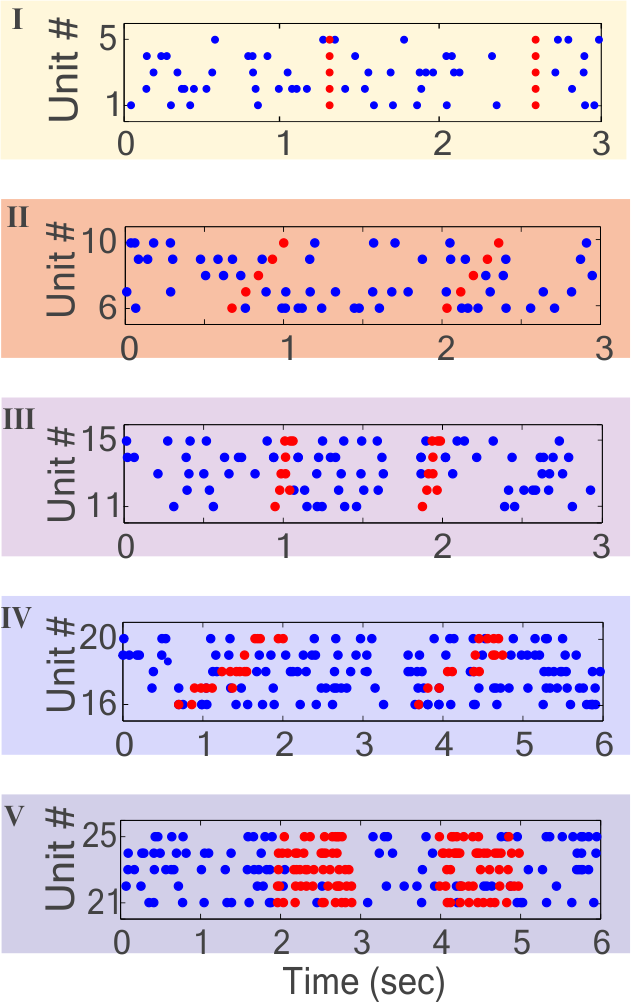
\includegraphics[scale=0.3]{figures/CellAssembliesZoom.png}
    \caption{Adapted from \cite{RussoDurstewitz}. Different cell assembly realizations, resulting from different definition of temporal precision and coordination.}
    \label{fig:CellAsseDet}
\end{figure}
The method we used does not limit to focus on a single specific assembly concept, theoretical idea, or particular time-scale. Instead it treats the temporal scale, precision, and internal organization of coherent activity patterns as free parameters, to be determined from the data, and is thus is free to detect a large family of possible assembly definitions at any time scales and spike coordination.\\
The the assembly detection method presented is based on a statistical approach, starting from the idea that any assembly recurs as repetition of activity patterns in a set of simultaneously recorded spike trains. As shown in figure\ref{fig:CellAsseDet} a pattern of activity can be anything from synchronous and precise spike activity ($lag = 0$) to delayed spike activity ($lag\neq 0$), to broader scale of firing rate.\\Usually an arbitrary width $\Delta$ for binning the spike time series is chosen, compromising the possibility to detect any temporal scale. The idea proposed in \cite{RussoDurstewitz} is instead to capture the multiplicity of temporal scales mentioned above introducing a set of widths $\Delta \in \{\Delta_{min},...,\Delta_{max}\}$, and retain the characteristic temporal scale of a formed assembly using a statistical test.\\The method is conceptualized as indirect proof of not independence of the activity of units composing the assembly.\\At the first step the algorithm detects dependent pairs of units, from which high order assemblies are recursively build up using an agglomerative procedure. The mathematical formalization starts from the definition of joint probability of two independent samples.\\For two independent units with stationary spike trains, the joint distribution of spike occurrences at a specified time lag $l$ would factor into the single unit ($'$marginal$'$) distributions, $p(A,B)=p(A)p(B)$.\\ Assume each recorded spike time series has been converted into a series $\{c_t\}$ of spike counts of length T at bin width $\Delta$, with $\# A$ and $\# B$ denoting the total numbers of spikes emitted by units A and B, respectively. If $\Delta$ is small enough such that $c_t\in\{0,1\}$ (binary counts), then, under the null hypothesis ($H_0$) of independence, the joint spike count $\#_{AB,l}$ at time lag $l$ follows a hypergeometric distribution with mean $\mu_{AB,l}=\# A \# B/(T-l)$ and variance $\sigma^{2}_{AB,l}$. If the binning is such that spike counts $c_t$ larger than one occur, the hypergeometric distribution is no longer directly applicable. In this case the series are split into several (mutually dependent) binary series for which is still possible to derive a joint mean and variance (see Materials and Methods session of \cite{RussoDurstewitz}).\\To proceed with the indirect proof one has to check for deviation from the null hypothesis of independence $H_0$ at lag $l$. At this point the developers of the methods notice that, since non-stationarities could corrupt the joint mean and variance, they can not be used for the proof. Instead to used classical strategy for correcting non-stationarity such us sliding window (\cite{Gruen}) or bootstrap-based method (\cite{Fujisawa}, \cite{Pipa}, \cite{Picado}), which imply considerable computational burden, they alternatively suggest a new simple remedy for non-stationarity based on difference in counts $\#_{ABBA,l^-} \equiv \#_{AB,l^-} - \#_{AB,l^*}$ that subtract from each joint spike count $\#_ {AB,l^-}$ the number $\#_{AB,l^*}$ of occurrences of the reference pattern $(A,B)_{l^*}$. In \cite{RussoDurstewitz} is discussed in depth the choice of the reference lag $l^*$.
The statistic $Q_{AB,l}\equiv \#_{ABBA,l^2}/\hat{\sigma}_{ABBA}^2$ is approximately F-distributed and can be used for fast parametric assessment of the null hypothesis. It is important to notice that difference statistic corrects for non-stationarity artifacts and diminish the computational load of the algorithm. This makes possible the test of multiple bin sizes. The whole procedure is repeated for a set of user-provided bin widths $\Delta \in \{\Delta_{min},...,\Delta_{max}\}$. For each formed assembly, the width $\Delta^*$ associated with the lowest p-value is defined as its temporal precision or its typical time scale.

{\color{red} La seconda parte e' copiata da eleonora. Rivedi}
Both the dynamic nature of the task and the complex network of direct and indirect pathways
connecting basal ganglia and VTA make cell assembly analysis particularly suited to investigate
the neuronal correlates behind reinforcement learning. First, by explicitly correcting for non-
stationarity, CAD can account for the quick changes in network states, typical of reversal
learning. Second, while cell assemblies are often detected by aligning the population activity to
task/behavioral events, CAD sums evidence of assembly activity throughout the task and
session. In this way, the same assembly can be detected even if it changes its time of activation
within the trial (e.g. moving from reward to the conditioned stimulus (CS+) onset, once built the
stimulus–reward association). Third, by selecting among all assemblies those composed by
units of different brain regions, one can specifically target inter-regional interactions.
%The mean μAB,l and variance σ2AB,l could, in principle, be used to check for deviation from the H0 of independence at lag l, but in practice such a statistic would be corrupted by non-stationarities like (coupled) changes in the underlying firing rate (see Materials and methods, Figure 7, and Appendix on the importance of accounting for non-stationarity). Sliding window (Grün et al., 2002b) or bootstrap-based (Fujisawa et al., 2008; Pipa et al., 2008; Picado-Muiño et al., 2013) analyses have most commonly been used to deal with this issue, but come at the price of considerable data loss or computational burden. Here we suggest a simple remedy which corrects for non-stationarity locally by using the difference statistic #ABBA,l=#AB,l−#AB,−l (see Materials and methods, Figure 6B). The idea is that this way non-stationarities in firing rates would cancel out locally, on a comparatively fine time scale (≈lΔ), since they would affect #AB,l and #AB,−l alike (for assessment of synchronous spiking, we use #ABBA,0=#AB,0−#AB,l∗, with l∗=−2; see sect. ‘Choice of reference (correction) lag’ for the motivation of this particular choice and a more general discussion of the reference statistics chosen). The statistic Ql≡#ABBA,l2/σ̂ 2ABBA,l finally is approximately F-distributed and can be used for fast parametric assessment of the H0 (see Materials and methods and Figure 7; Figure 7—figure supplements 1 and 2, for derivation and empirical confirmation using non-stationary synthetic data).

%Having derived a fast, non-stationarity-corrected parametric test statistic for assessing the independence of pairs, we designed an agglomerative, heuristic clustering algorithm for fusing significant pairs into higher-order assemblies (see Figure 6—figure supplement 1 and Materials and methods for full derivation and pseudo-code). In essence, at each agglomeration step the algorithm treats each set of units fused in an earlier step just like a single unit with activation times defined through one of its member units. This allows for the same pair-wise test procedure on sets of units as defined for single units above, while at the same time effectively testing for higher-order dependencies based on the joint (set) distributions (see Materials and methods). Each pair is tested at all possible lags l∈{−lmax…lmax} (with lmax provided by the user), which is a reasonably fast process given the parametric evaluation introduced above. Should a pair of unit-sets prove significant at several lags l at any step, only the one associated with the minimum p-value is retained. The recursive set-fusing scheme stops if no more significant relationships among agglomerated sets and single units are detected. All subsets nested within larger sets are then discarded. This whole procedure is repeated for a set of user-provided bin widths Δ∈{Δmin…Δmax}. For each formed assembly, the width Δ∗ associated with the lowest p-value may then be defined as its characteristic temporal precision. All tests are performed at a user-specified, strictly Bonferroni-corrected α-level (always set to 0.05 here; see Materials and methods for details).